\documentclass[rnd]{mas_proposal}
% \documentclass[thesis]{mas_proposal}

\usepackage[utf8]{inputenc}
\usepackage{amsmath}
\usepackage{amsfonts}
\usepackage{amssymb}
\usepackage{graphicx}

\title{Interactive Short Answer Grading}
\author{Mohandass Muthuraja, Jeeveeswaran Kishaan}
\supervisors{Prof. Paul G. Ploeger\\Deebul Nair }

% \thirdpartylogo{path/to/your/image}

\begin{document}

\maketitle

\pagestyle{plain}

\chapter{Introduction}
\begin{itemize}
    \item An introduction to the general topic you are covering.
    \item Why is it important? \\
     Active learning is a new paradigm of learning where the learner queries the user/a human for the labels of certain data samples in such a way that it can learn to produce the desired outputs with higher accuracy. By actively selecting the data samples to label, it reduces a considerable amount of labeled training samples, thus, alleviating the problem of insufficient labelled data which is prevalent in supervised learning approaches. \\
     The effectiveness of an active learning approach heavily depends upon the following factors:
     \begin{itemize}
     \item Instance selection - selection of the unlabeled data samples for the user to label is arguable one of the most important factors in active learning. While choosing the most informative samples can improve the performance, poor selection can pave the way for unforseen degradations. Some of the most common methods used for sampling include:
     \begin{itemize}
     \item Entropy sampling
     \item Boosted Entropy Sampling
     \item Margin Sampling
     \item Diversiy Sampling
     \item Representativeness sampling
     \end{itemize}
     \item Seed selection - The initial set of labeled training data samples which is used to train the first classifier is known as seed. It has been showed that the quality of this seed plays a key role in the effectiveness of Active learning algorithms.

	\item Batch size - The number of samples labeled at each iteration of Active learning is defined by the batch size. A balanced batch size has to be identified between a small batch size (which might not account for the lexical diversity) and a large batch size (which might contain many similar and redundant samples). Variable batch size has been proposed as a solution for this in one of the recent work.
	
     \end{itemize}
    
Interactive short answer grading \\

Short answers typically consist of one to few sentences. Many approaches have been suggested to automate the task of grading short answers. Most of the approaches learn a model which can grade the students' answers based on the similarity of them with the correct answer provided by the professor / instructor. This research and development project deals with making the automatic short answer grading interactive, which involves a human in the loop to direct the learner in the correct way towards making the correct prediction of grades for a given answer. Active learning seems to be the best choice for this task as it actively queries the human for the grades of the samples it is most uncertain of. This approach is focussed on saving the time, cost and bias of manual grading by reducing the effort of a human in grading tasks by choosing only the best samples to be graded rather than the whole answer sheet. 

\end{itemize}





\section{Problem Statement}
\begin{itemize}
    \item What are you going to solve?
    \item How are you evaluating?
    
    \item One of the biggest challenge involved in supervised learning in the need for large datasets. Generating a large data for short answer grading is also an obstacle. Many automatic short answer grading systems rely on supervised learning techniques. This, in turn, leads to high annotation cost of labeling the large training data. Also, the workload for labeling the data is more.
    \item As new data are generated on a regular basis, retraining the model for every new data also have a caveat of high computation cost.  Developing a generic model to overcome the deficit of retraining the model for every new answer can solve this issue.
    \item Short answer grading typically does not look for grammatical correctness and coherency. Short answers written by students have a lot of lexical diversity. Active learning can be used to handle the lexical diversity by involving human in training the model.
\end{itemize}


\chapter{Related Work}
\begin{itemize}
    \item What have other people done?
    \item Why is it not sufficient?
\end{itemize}

\section{Section 1}
\section{Section 2}



\chapter{Project Plan}

\section{Work Packages}
The bare minimum will include the following packages:
\begin{enumerate}
    \item[WP1] Literature Search
    \item[WP2] Experiments
    \item[WP3] Project Report
\end{enumerate}
Keep in mind that depending on your project, you will probably need to add work packages that are more suited to your projects.

\section{Milestones}
\begin{enumerate}
    \item[M1] Literature search
    \item[M2] Experimental setup
    \item[M3] Experimental Analysis
    \item[M4] Report submission
\end{enumerate}

\section{Project Schedule}
Include a gantt chart here. It doesn't have to be detailed, but it should include the milestones you mentioned above.
Make sure to include the writing of your report throughout the whole project, not just at the end.

\begin{figure}[h!]
    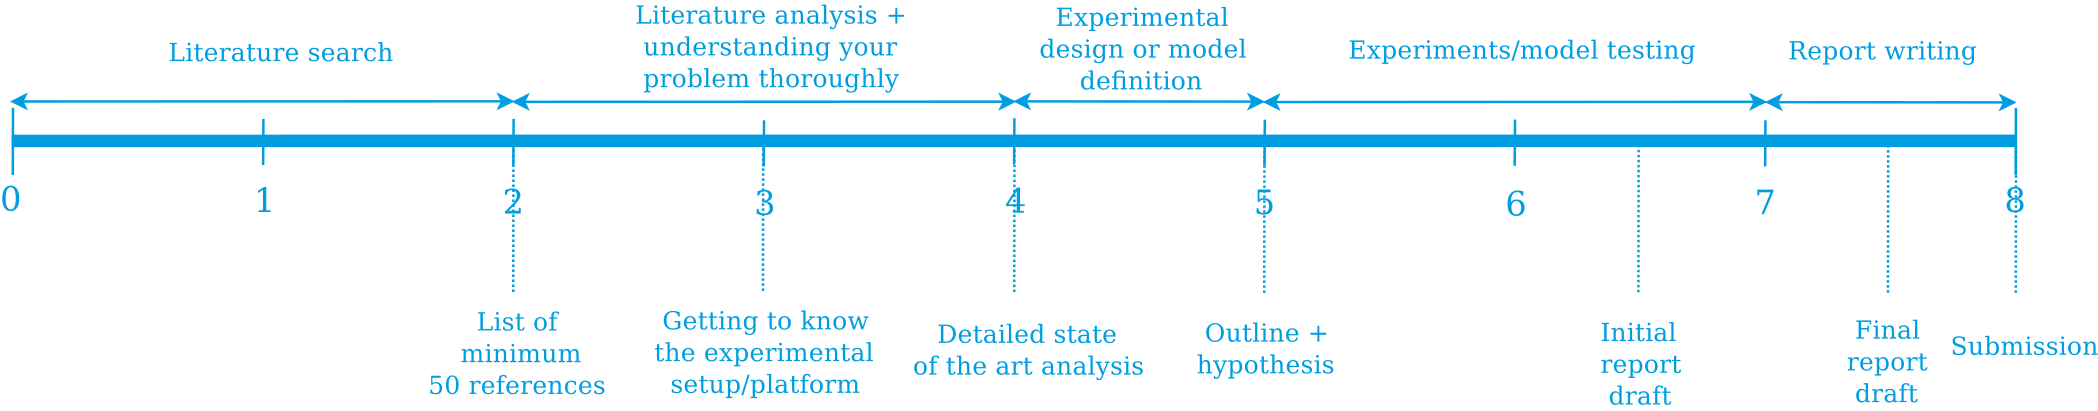
\includegraphics[width=\textwidth]{rnd_deliverable_timeline}
    \caption{}
    \label{}
\end{figure}

\section{Deliverables}
\subsection{Minimum Viable}

\begin{itemize}
    \item Survey
    \item Analysis of state of the art
    \item Simple simulated use case
    \item Demo on youBot or Jenny
\end{itemize}

\subsection{Expected}
\begin{itemize}
    \item Comparation of approaches in the robot
\end{itemize}

\subsection{Desired}
\begin{itemize}
    \item Integration to scenario
\end{itemize}


\nocite{*}

\bibliographystyle{plainnat} % Use the plainnat bibliography style
\bibliography{bibliography.bib} % Use the bibliography.bib file as the source of references




\end{document}
